\begin{filecontents*}{auden.tex}
\begin{verse}
Look, stranger, on this island now \\
The leaping light for your 
delight discovers, \\
Stand stable here \\
And silent be, \\
That through the channels of the ear \\
May wander like a river \\
The swaying sound of the sea. 
\end{verse}
\end{filecontents*}

\documentclass[a4paper,amsmath]{oblivoir}

\usepackage{fapapersize}
\usefapapersize{*,*,1in,*,1in,*}

\makeatletter
\let\ATonum\@onum
\makeatother

\usepackage[hcr]{kstextks}    %%% install ksmisc package from KTUG Private Repo
%\usepackage{esgutil}
\usepackage{refcount}
\usepackage{ob-mathleading}
\ifxetex
\usepackage[normalem]{ulem}
\fi

\input{insbox}
\usepackage{lipsum}
\usepackage{manfnt}
\usepackage{etoolbox}
\usepackage{filecontents}
\let\bs\relax
\usepackage{latexdemo}

\usepackage{xcolor}
\usepackage{efbox}
\usepackage{graphicx}
\usepackage{hologo}
\usepackage{relsize}
\usepackage{tcolorbox}
\tcbuselibrary{minted,breakable}
\tcbset{listing engine=minted,colframe=cyan,colback=cyan!5!white}

\setmainfont{TeX Gyre Pagella}
\setsansfont{Noto Sans}
\setmonofont{Noto Sans Mono}
\setkomainfont(Noto Serif CJK KR)(* Bold)(Noto Sans CJK KR)[CharRaise=-.0125em]
\setkosansfont[Noto Sans CJK KR]()( Bold)( Medium)
\usepackage{unicode-math}
\setmathfont{texgyrepagella-math.otf}

\newcounter{sub}
\newcommand\bangotsuite{\stepcounter{sub}\thesub}

\usepackage{tikz}
\newcommand\tikzlogo{Ti\textit{k}Z}
\usetikzlibrary{shadows}

\setlength{\parindent}{0mm}

\newcommand\pkg[1]{\textsf{#1}}

\ExplSyntaxOn 

\NewDocumentEnvironment {intro} {o}
{
    \IfValueTF { #1 }
    {
        \int_set:Nn \l_tmpa_int { #1 }
    }
    {
        \int_set:Nn \l_tmpa_int { 1 }
    }
    \noindent \rule {\linewidth}{3pt}
    \par 
    \sffamily [No.\space\int_use:N \l_tmpa_int ]\ \ 
    \bfseries
}
{
    \hfill \underline{\hphantom{2019}}년~\underline{\hphantom{06}}월~ \underline{\hphantom{25}}일 
    \par 
    \vskip -.3\baselineskip 
    \noindent \rule {\linewidth }{1pt}
    \par 
    \vskip .5\baselineskip 
}

\NewDocumentCommand \exverb { d|| }
{
    \texttt { \tl_to_str:n { #1 } }
}

\ExplSyntaxOff 

\NewDocumentEnvironment {questiona} { m }
{
%    \medskip
    \begin{tcolorbox}[title={#1},fonttitle={\sffamily\bfseries}]
}{%
    \end{tcolorbox}
}

\NewDocumentEnvironment {questionp} { }
{
%    \medskip
    \begin{tcolorbox}[colframe=orange!30!black!60,colbacktitle=orange!25!gray,
    title={연습문제},fonttitle={\sffamily\bfseries}]
}{%
    \end{tcolorbox}
}


\NewDocumentEnvironment {exampleonly} {}
{%
%    \begin{tcblisting}{listing only}
    \par
    \singlespacing \vskip-.5\onelineskip
    \expandafter\tcblisting{listing only,breakable,before={\par\medskip\setstretch{1}}}
}{
    \endtcblisting
%    \end{tcblisting}
}

\NewDocumentEnvironment {exampleside} {}
{%
    \par
    \singlespacing \vskip-.5\onelineskip
    \tcblisting{listing side text,righthand width=.35\textwidth,breakable}%
}{%
    \endtcblisting
}

\NewDocumentEnvironment {examplebelow} {}
{%
    \par
    \singlespacing \vskip-.5\onelineskip
    \tcblisting{breakable}%
}{%
    \endtcblisting
}
%\newtcblisting{examplebelow}{breakable,before={\par\medskip\setstretch{1}}}

\begin{document}

\begin{intro}[8]
Stand stable here
\end{intro}


\begin{questiona}{문제}
두 개의 박스를 잇대어서 왼쪽에는 \LaTeX{} 소스의 입력을
오른쪽에는 그 출력 결과를 보여주는 \texttt{myexample} 환경을 만들어보아라.
\end{questiona}

\section{file}

\LaTeX 의 성공 요인은 여러 가지가 있지만 맨처음 등장했을 때 사람들을 매료했던 것이
목차와 상호참조의 자동생성 기능이었다. 세상에 태어나니까 이미 Microsoft \textsc{Word}가
존재했던 사람들이야 이해하기 어렵겠지만 이 때가 1980년대였음을 상기하자.

\subsection{aux, toc, lot, lof라는 파일}

\texttt{latex}({\small 앞으로 \texttt{xelatex}이나 \texttt{pdflatex} 등 실행 명령을 가리킬 때
\texttt{latex}이라고 지징한다})을 실행하였을 때 여러 가지의 부수파일이 만들어지는데
그 가운데 확장명이 \verb|.aux|인 것이 있다. \texttt{latex}이 실행하면서 이런저런 정보들을
적어둔 파일이다. 여기에는 장절의 번호, 표제, figure/table의 캡션과 번호, \verb|\label|들에 대한
정보 등을 담고 있다. 
다음 번 \texttt{latex} 실행 시에 이 정보를 읽어와서 참조와 (\textsf{hyperref}의 도움을 받아서)
하이퍼링크 등을 만들어낸다. table of contents는 \verb|aux| 이외에 \verb|toc|와 \verb|out|이라는 
다른 파일을 더 이용하므로 (\verb|out|은 주로 pdf bookmark를 만드는 데 쓴다) \verb|aux|만으로 이루어지는 것은 아니지만 관련된 정보는 담고 있다.
\verb|\includeonly| 명령을 써서 chapter 2만 조판하려 할 적에 조판되지 않는 chapter 1의 
마지막 페이지 번호 같은 것은 \verb|aux|에서 가져오는 것이다. (따라서 chap1.aux라는 파일이
없으면 2장의 시작 페이지가 제대로 조판되지 않고 chapter 1에 있는 참조 정보도 활용할 수 없다.)

그러니 \verb|.aux| 파일은 웬만하면 지우지 말자. 실행 오류 때문에 초기화 컴파일이 필요할 때를 제외하고.

\verb|toc|, \verb|lof|, \verb|lot| 확장자를 갖는 파일들은 각각 목차, 그림 목차, 표 목차를
넣어두고 있는 파일들이다. \verb|\tableofcontents| 같은 명령이 불릴 적에 여기에 기록된 정보를 가지고
목차를 만든다. 

이 파일들에 뭔가를 임의로 적어넣는 것이 가능하다. 아무거나 적어넣으면 이상한 결과를 보게 될 것인데
예컨대 \verb|toc| 파일은 
\begin{verbatim}
\contentsline {section}{Introduction}{1}{section.0.1}
\end{verbatim}
과 같은 행들로 이루어져 있다. 이 파일과 상호작용하기 위한 명령 \verb|\addtocontents|나 
\verb|\addcontentsline| 따위가 미리 정의되어 있고 이에 대한 설명은 예컨대 memoir 매뉴얼에
상세하다. 그러므로 이 명령이나 파일들에 대해서 여기서 더 말하지 않으려 한다.

외부 파일을 이용하는 \LaTeX 의 기능으로 index(색인)과 bibliography가 더 있다. index에
대해서만 말해보자면, \verb|\index|라는 명령이 주어지는 순간에 그 인자와 현재 위치를
\verb|.idx|라는 파일에 쓴다. 한 번 컴파일이 끝나고 나면 \verb|.idx| 파일에는
그 소스에 나온 모든 \verb|\index| 엔트리들을 저장하고 있다.

\verb|makeindex|라는 프로그램은 \verb|.idx|를 읽어서 일단 정렬하고 식자할 수 있는 형태로
만들어서 \verb|.ind| 파일에 저장한다. 이 때에 “스타일”이라고 하는 것을 적용하는데 이 스타일
파일은 \verb|makeindex|가 이해하는 언어로 작성되어 있어야 한다. 보통 \verb|.ist|라는
확장명을 갖는다. 아무튼 이 과정은 \verb|latex|이 관여하는 것이 아니다.
\verb|latex|은 만약 \verb|.ind| 파일이 있으면 그 내용 전체를 \verb|\printindex|
명령이 불린 위치에 그대로 삽입한다.
\verb|komkindex|는 한글 UTF-8 문자열도 처리가 가능하도록 한 \verb|makeindex| wrapper이다.
한글이 문제가 되면 \verb|komkindex|를 쓰는 이유는 거기에 있다. 최근 \verb|makeindex|를
대체하기 위한 노력들, 예컨대 \verb|xindy|, \verb|xindex| 등이 개발되는 중에 있지만
핵심 개념은 이에서 벗어나지 않는다.



\subsection{verbatim이라는 것}

verbatim [{\fontspec{HCR Batang LVT}və\textkslongvowelmark\,rbéɪtəm}]은 lshort을 읽었다면 다 알고 있을 것으로 본다.
\LaTeX 에 관한 \LaTeX{} 문서를 작성하려면 부득이하게 verbatim으로 떡칠(\ldots)된 소스를 만들 수밖에 없다.
verbatim에 대하여 반드시 기억해두어야 할 것은, 이것이 “more fragile than fragile”이라는 사실이다. 
verbatim 텍스트는 일단 verb 상태가 되고 나면 다른 명령의 인자로 사용될 수 없다. 각주에도 들어갈 수 없고, 장절 명령과 같은 moving arguments에도 들어가지 못한다.
verbatim 내부에서 명령을 통한 조작을 가할 수도 없다.
그래서 일찍부터 verbatim을 좀더 fancy하게 다루는 수많은 방법이 개발되어 있다. minted 패키지가 사용하는
fancyvrb 같은 것이 대표적이다. 아마도 \LaTeX{} 패키지 가운데 verbatim 관련이 종류가 많고 비슷한
것들도 많은 부류에 속할 것이다. 주로 Source Code Listing 관련하여 많은 요구가 있어왔기 때문이다.
이 패키지들은 위에 열거한 verbatim의 제약을 조금이라도 벗어나기 위한 몸부림이다.

expl3의 입장에서 말하자면 verbatim은 string과 비슷하다. 예를 들어

\begin{exampleside}
\ExplSyntaxOn
\ttfamily
\tl_to_str:n { \verbatim \l_tmpa_tl }
\ExplSyntaxOff
\end{exampleside}

이 예를 보면 typewriter font로 \verb|\tl_to_str:n|한 결과를 출력하면 그것이 verbatim이라는 것이다.
우리는 expl3의 막강한 arguments expansion 함수들을 이용하여 원하는 결과를 출력할 수 있다.

\begin{exampleside}
\ExplSyntaxOn
\ttfamily
\tl_set:Nn \l_tmpa_tl { And~silent~be }
\tl_to_str:n { \l_tmpa_tl } \\
\exp_args:No \tl_to_str:n { \l_tmpa_tl }
\ExplSyntaxOff
\end{exampleside}

그러나 expl3라 하더라도 verbatim 자체는 주의깊게 다루어야 한다는 사실을 기억하자. \textsf{xparse}의
\verb|v|형 인자는({\small expl3의 cs인자형의 \verb|v|와는 다른 것이다}) 다른 명령이나 함수에 인자로 넘겨주지 못한다는 제한은 이래서 생겨났다.

\subsection{example 환경 설계의 아이디어}

문제로 돌아와서 생각해보자. 한 번은 입력 형태이고 한 번은 조판된 형태를 보여야 하니까
왼쪽 박스에는 verbatim 텍스트가, 오른쪽 박스에는 그 조판 형태가 나와야 한다.
이것은 같은 소스를 한 번은 verbatim으로 다른 한 번은 입력 코드로 두 번을 읽어야 한다는 뜻이다.

단순, 명쾌, 무식하게 두 번 입력하여 이런 비슷한 것을 만드는 것을 먼저 해보려 한다.

\begin{examplebelow}
\begin{minipage}{.5\textwidth}
\begin{verbatim}
\begin{verse}
Look, stranger, on this island now \\
The leaping light for your 
   delight discovers, \\
Stand stable here \\
And silent be, \\
That through the channels 
   of the ear \\
May wander like a river \\
The swaying sound of the sea. 
\end{verse}
\end{verbatim}
\end{minipage}%
\begin{minipage}{.5\textwidth}
\begin{verse}
Look, stranger, on this island now \\
The leaping light for your 
delight discovers, \\
Stand stable here \\
And silent be, \\
That through the channels of the ear \\
May wander like a river \\
The swaying sound of the sea. 
\end{verse}
\end{minipage}
\end{examplebelow}

똑같은 텍스트를 두 번 쓰면 문제가 되는 것이 귀찮을 뿐더러 둘 중 하나만
나중에 수정하게 될 수도 있다는 점이다. 단일 소스를 두 번 읽을 수 있으면 좋겠다.
여기 식자할 내용 전체를 외부의 어떤 파일에 write해두었다가
그 파일을 mode를 달리하여 두 번 읽으면 되지 않을까?

\subsection{input과 include}

이미 파일이 있다고 하자. 이것을 읽어오는 방법은 무엇인가?

\verb|\input|이라는 primitive는 외부 파일을 통째로 읽어와서 그 명령이 불린 위치에
그대로 삽입해준다. verbatim으로 읽어오는 것이 아니라는 점을 알아두어야 한다.
매크로는 들어와서 그대로 실행되고 주석문은 무시된다.

참고로 \LaTeX 의 \verb|\include|라는 명령이 있는데 이것은 용도가 완전히 다르다.
이것은 주로 긴 \LaTeX{} 문서를 부분별로 작성하려 할 때 쓰는 것으로 \verb|\include|되는
파일은 \verb|\documentclass|가 없는 파일이어야 하고 문서의 본문에서 불려야 하며
부수 정보(\verb|.aux|)를 함께 불러오고 항상 새로운 페이지로 시작한다.
\verb|\includeonly|는 본문에 출현할 \verb|\include| 명령을 일부 활성화/무시할 수 있게
해주는 것이다. 당연히 원시 명령인 \verb|\input|에는 그런 거 없다.

어디에 있는 파일을 불러올까? 오늘날 우리가 쓰는 \TeX\,Live와 같은 텍 시스템은
\verb|kpathsea|라는 라이브러리에 기대어 컴파일되어 있다. 이 말은 \verb|kpathsea|가
그 위치를 알려줄 수 있는 파일이면 모두 \verb|\input|할 수 있다는 의미이다.
현재의 작업 폴더와 그 상대위치로 지정된 파일, \verb|TEXMF/tex| 위치
아래의 파일은 다른 조치없이 바로 \verb|\input| 가능하다.
상대 위치를 path로 주는 경우에 Windows 시스템이라도 path 경로는 반드시 \verb|/|로
주어야 한다. 작업 폴더 아래 \verb|texts|라는 하위 폴더를 만들고 그 안에
\verb|testa.tex|이라는 파일이 있을 때,
\begin{verbatim}
\input{texts/testa.tex}
\end{verbatim}
으로 하면 운영체제에 상관없이 모두 잘 불러올 것이다.

\hologo{plainTeX}의 \verb|\input| 명령과 \LaTeX 의 \verb|\input| 명령은
거의 같지만 한 가지가 다른데 \LaTeX 의 것이 “중괄호 인자”를 쓸 수 있다는 것이다.
\begin{verbatim}
\input inputfile.tex
\input{inputfile.tex}
\end{verbatim}
아래쪽 것이 \LaTeX{} 방식이다. 이 \LaTeX{} 명령의 편리한 점 하나는 확장자가 \verb|.tex|인
파일은 파일 이름만 써도 된다는 것이다.


\subsection{verbatiminput}

그런데 \verb|\input|은 파일의 contents를 “입력파일”로 읽어온다. 이래서는 verbatim으로
표현할 수가 없다. 심지어
\begin{verbatim}
\verb+\input{auden.tex}+
\end{verbatim}
이런 명령은 어떤 방법으로도 \verb|auden.tex|이라는 파일의 내용을 \verb|\verbatim|의
인자로 만들 수 없다. 위의 것은 그냥 \verb|\input{auden.tex}|이라는 글자를 찍어줄 뿐이다.

이 문제 해결에 관련된 기나긴 역사를 요약하려면 별도의 글이 필요하다. 우리는 이왕에 memoir 
클래스를 쓰고 있으므로 memoir가 이미 이 문제를 간단히 해결해두고 있다는 점을 지적하고 지나가려 한다.

\begin{verbatim}
\verbatiminput
\boxedverbatiminput
\end{verbatim}

이에 대한 상세한 설명은 memoir 매뉴얼을 보자.

\begin{verbatim}
\boxedverbatiminput{auden.tex}
\end{verbatim}

\boxedverbatiminput{auden.tex}

\subsection{잠정적 해결}

\begin{examplebelow}
\ifvmode\leavevmode\fi
\begin{minipage}{.5\textwidth}
\verbatiminput{auden.tex}
\end{minipage}
\begin{minipage}{.45\textwidth}
\input{auden.tex}
\end{minipage}
\end{examplebelow}

\verb|\boxedverbatiminput|은 다른 환경 안에 들어가기 어렵다. 그래서 \verb|\verbatiminput|만을
썼는데 일단 소스와 결과를 나란히 놓는 것까지는 어떻게든 해본 셈이다.

이제 주어진 텍스트를 어떻게 “임의의 파일”에 쓸 것인가가 남았다.

\section{외부 파일에 쓰기}

\subsection{stream과 file}

파일 조작의 기본은 다음과 같다.
\begin{enumerate}[(1)]\firmlist
\item 파일을 연다. 이것은 운영체제에게 특정 (물리)파일의 내용을 전달해달라고
요청하는 것이다. 이렇게 해서 전달받은 파일의 내용을 \textit{stream}에 연결해둔다.
열기는 “읽기 위해 열기”와 “쓰기 위해 열기”가 있다.
\item \verb|latex|은 오로지 stream만을 조작한다. “쓰기 위해 연” stream에는
아무 것도 없는 것이 기본이므로 만약 파일 내용을 수정하려면 “읽기 위해 열고”
그 내용을 (텍스트 파일에서 주로 한 행씩) 수정하여 “쓰기 stream”으로 보내어야 한다.
\item stream 조작이 끝나면 이 파일을 닫는다. “쓰기 위해 연” stream은
파일이 닫히는 순간 OS는 stream의 내용을 그대로 물리 파일로 쓴다.
\end{enumerate}

파일 조작에서 가장 중요한 것은 열고 닫는 것이다. 열린 stream은 반드시 닫아주어야 한다.
\verb|latex|은 실행을 시작할 때 main aux라고 부르는 \verb|.aux|를 
“읽기 위해” 연다. 그리고 같은 파일을 “쓰기 위해” 열고
컴파일이 끝나면 이것을 닫는다.  즉, 기존에 \verb|.aux|에 
쓰여 있던 내용들이 “읽기”로 모두 들어오고, 컴파일하면서 생성되는 정보는 “쓰기”가 이루어진다.
“쓰기”로 읽었기 때문에 이 파일 자체는 이전 내용과 상관없이 완전히 새롭게 쓰여지는데 
이전 내용이 이미 읽어진 후이기 때문에 “이전 내용이 반영되어 변경되는 것처럼” 보이는 것이다.

“즉시 쓰기” (immediate write)라는 것이 있다. 이것은 (그 레지스터 번호를 사용자가 알 필요가
없는) 어떤 stream으로 주어진 file을 연결하여 열고 주어진 인자를 그 stream으로 보낸 다음
즉시 file을 close하는 일을 한다. stream이 열려 있지 않고 새로이 열고 바로 닫는 것이기
때문에 이 명령이 여러 번 불리면 그 때마다 파일 내용이 변경되어 이전 내용이 보존되지 않는다.

원칙적으로 stream으로 보내기는 other로 이루어진다. 즉 verbatim으로 보내는 것이다.
그러나 \LaTeX 이 stream으로 보내면서 “매크로가 확장된 이후에” 보내면 명령이 풀리거나 실행된
상태가 저장될 것이고 “매크로를 확장하지 않고 있는 그대로” 보내면 verbatim 쓰기가 될 것이다.
“쓰기”에서는 항상 “언제 확장할 것인가”가 매우 중요하다.

\subsection{filecontents 환경}

예전부터 사용된 “파일 쓰기” 대표적인 것이 \texttt{filecontents} 환경이다.
\LaTeX{} 자체가 제공하는 환경이고 오랜 역사를 자랑한다.
이 환경은 \verb|\documentclass| 명령 이전에 써야 하고 파일 이름을 인자로 줄 수 있으며
환경 안의 내용이 verbatim으로 저장된다. 만약 같은 이름의 파일이 존재한다면 아무 일도 일어나지 않으므로
새 파일을 만드는 것만 가능하다. 한편 별표를 붙인 환경은 이 파일에 붙는 간단한 기록 정보를
나타내는 주석문(\%로 시작하는 행)을 제외하고 쓴다.

이 환경은 주로 한 개의 파일에 스타일 파일을 같이 넣어서 전달하거나 할 때 쓰였다.

위에 언급한 제약을 조금 완화하여 본문 어디에서나 사용할 수 있도록 
수정한 \textsf{filecontents} 패키지가 있다.
원래 아래 보기는 \verb|\documentclass| 이전에 두어야 하지만 이 패키지의 도움을 받아
여기 예제를 작성해본다.

\begin{exampleonly}
\begin{filecontents}{mytest1.tex}
\begin{verse}
Look, stranger, on this island now \\
The leaping light for your delight discovers, \\
Stand stable here \\
And silent be, \\
That through the channels of the ear \\
May wander like a river \\
The swaying sound of the sea. 
\end{verse}
\end{filecontents}
\end{exampleonly}

\begin{filecontents}{mytest1.tex}
\begin{verse}
Look, stranger, on this island now \\
The leaping light for your 
   delight discovers, \\
Stand stable here \\
And silent be, \\
That through the channels 
   of the ear \\
May wander like a river \\
The swaying sound of the sea. 
\end{verse}
\end{filecontents}


현재 폴더에 \verb|mytest1.tex|이 생겨나 있는지 확인하여라. 이것을 \verb|\boxedverbatiminput|하면

\boxedverbatiminput{mytest1.tex}

위와 같이 된다. 처음의 주석문 4줄을 붙이지 않으려면 \verb|filecontents*| 환경 안에 넣는다.

예전부터 전해내려오는 주의사항 중에 “filecontents의 인자인 파일 이름을 현재 작성중인 문서 파일의 이름과 같게 하지 말라”는 것이 있다. 생각해보면 어차피 filecontents 환경은 같은 이름의 파일이 있으면 아무 일도 
하지 않으니까 결과적으로 아무 일도 일어나지 않겠지만 코딩 오류인 것은 틀림없다.



\subsection{memoir의 file 관련 명령}

memoir는 파일을 다루는 명령이 기본적으로 제공한다. 관련 내용은 매뉴얼을 참고하고 우리가 필요한 부분만
살펴보겠다. 특히 읽어오기에 관한 부분은 생략한다.

\begin{exampleonly}
\newoutputstream{<stream>}
\openoutputfile{<filename>}{<stream>}
\addtostream{<stream>}{text}
\closestream{<stream>}
\end{exampleonly}

설명이 필요없을 것이다. \verb|\addtostream| 명령은 \texttt{text}로 오는 부분을 “미리 확장해서”
stream으로 보낸다.

\begin{examplebelow}
\newoutputstream{outputone}
\openoutputfile{mytest1.tex}{outputone}
\def\myname{Nova de Hi.}
\addtostream{outputone}{\myname}
\closeoutputstream{outputone}

\verbatiminput{mytest1.tex}

\fbox{\input{mytest1.tex}}
\end{examplebelow}

반면, 일절 확장하지 않고 verbatim으로 쓰는 데는 두 가지 방법이 있는데 하나는 열려 있는 stream에
내용을 추가해갈 수 있는 \verb|writeverbatim| (stream) 환경이고 다른 하나는 즉시 쓰기를 실행하는
\verb|verbatimoutput| (filename)이다. 따라서 \verb|verbatimoutput| 환경의 경우 다음 번에 실행되면
이전 내용은 사라진다.

memoir뿐 아니고 \textsf{tcolorbox}가 이용하고 있는 \textsf{listings}나 \textsf{sverb}
\textsf{example-p} 등의 비슷한 기능을 제공하는 패키지들이 모두 verbatim으로 쓰고 읽기를
지원하고 있다.

memoir의 file 관련 명령을 이용하여 원래 우리가 하고자 했던 것을 해보자.

\begin{examplebelow}
\newoutputstream{myout}
\openoutputfile{\jobname-test.tex}{myout}

\begin{writeverbatim}{myout}
\begin{verse}
Look, stranger, on this island now \\
The leaping light for your
delight discovers, \\
Stand stable here \\
And silent be, \\
That through the channels of the ear \\
May wander like a river \\
The swaying sound of the sea. 
\end{verse}
\end{writeverbatim}

\closeoutputstream{myout}

\noindent
\begin{minipage}{.5\textwidth}
\verbatiminput{\jobname-test.tex}
\end{minipage}%
\begin{minipage}{.5\textwidth}
\input{\jobname-test.tex}
\end{minipage}
\end{examplebelow}

\section{expl3의 \textsf{file}}

expl3는 단순히 verbatim을 읽고 쓰기 위한 환경들과는 달리 좀더 섬세하게 파일을
조작할 수 있도록 해준다.
expl3에서 파일 관련 제공하는 것은 세 종류가 있다.
하나는 파일로부터 “읽어오기” 위한 함수들로서 \verb|\ior_...|로 시작한다.
다른 하나는 파일에 “쓰기” 위한 함수들로서 \verb|\iow_...|로 시작한다.
그리고 \verb|\file_...|은 파일의 경로, 존재여부, 비교 등을 위한
함수를 제공한다.

파일 읽기에 대하여 조금 말해둔다. \verb|\input{<filename>}|과 같은 방법으로
파일이 존재하면 그 내용을 전부 input하는 것은

\begin{exampleonly}
\file_input:n { <filename> }
\file_if_exist_input:n { <filename> }
\end{exampleonly}

이 있다. 그런데 \verb|\ior_...| 읽기라는 것은 이처럼 파일 전체를 통째로 가져오는
것이 아니라 스트림으로부터 한 줄씩 처리하는 것을 기본으로 하는 것이다.

“읽기”를 위한 \verb|ior|과 “쓰기”를 위한 \verb|iow|를 다음과 같이 선언하는 것은
\begin{verbatim}
\ior_new:N
\iow_new:N
\end{verbatim} 
읽거나 쓰기 위한 스트림을 선언하는 것이다. (file에는 \verb|\l_tmpa_ior| 같은
스크래치 변수가 없다는 사실에 주의하자.)

이 스트림에 파일을 연결하여 여는 것은
\begin{verbatim}
\ior_open:Nn \l_inputfile_ior { file-to-read.txt }
\iow_open:Nn \l_outputfile_iow { file-to-write.txt }
\end{verbatim}
이렇게 한다. 

파일 작업이 종료되면 이를 닫아야 한다.
\begin{verbatim}
\ior_close:N
\iow_close:N
\end{verbatim}

“읽기”를 위한 조작을 보자. 기본적으로 한 줄(line)씩 읽어온다. 

\begin{exampleonly}
\ExplSyntaxOn
\ior_new:N \l_test_ior
\ior_open:Nn \l_test_ior { \jobname-test.tex }
\ior_get:NN \l_test_ior \l_tmpa_tl
\ExplSyntaxOff
\end{exampleonly}

앞서 저장한 파일 \verb|\jobname-test.tex|에서 처음 한 줄을 “입력 스트림으로 읽어서”
\verb|\l_tmpa_tl|에 저장하였다.
어떻게 읽느냐는 아주 중요한데 \verb|\ior_get:NN| 함수는 파일에 있는 토큰들을
normal token으로 읽는다. 그러나 \verb|\ior_str_get:NN|은 “string으로 (verbatim으로)
읽어서” \verb|\l_tmpa_tl|에 저장한다. \verb|_str_|가 붙은 함수는 모두
verbatim으로 읽는 것이다.

\verb|\ior_map_inline:Nn|은 파일을 끝까지 읽을 수 있게 한다. \verb|#1|은 현재 읽은
한 줄이다. 대응하는 \verb|\ior_str_map_inline:Nn|이 있다. 파일 읽기를 중간에 중단하려면
\verb|\ior_map_break:|를 쓴다.

\verb|\ior_if_eof:NTF|는 입력 스트림의 끝인가를 검사하는 것이다.

\begin{examplebelow}
\ExplSyntaxOn
\ior_new:N \l_test_ior
\ior_open:Nn \l_test_ior { \jobname-test.tex }
\ior_str_map_inline:Nn \l_test_ior
{
    \fbox { \sffamily\small \color{blue} #1 } \par
}

\ior_close:N \l_test_ior
\ExplSyntaxOff
\end{examplebelow}


쓰기 위하여 스트림을 여는 것은 앞서 보았다. 실제로 내용을 써넣는 것이 중요한데,
\begin{verbatim}
\iow_now:Nn
\iow_now:Nx
\end{verbatim}
이 둘 사이의 차이를 이해하는 것이 중요하다. \verb|:Nx| 쪽은 매크로가 있다면
확장한 다음에 스트림으로 보낸다.

\begin{examplebelow}
\ExplSyntaxOn
\iow_new:N \l_tmp_iow
\iow_open:Nn \l_tmp_iow { \jobname-testa.txt }
\iow_now:Nn \l_tmp_iow { \l_tmpa_tl{}~is~a~scratch~tl. }
\iow_close:N \l_tmp_iow

\verbatiminput{\jobname-testa.txt}

\tl_set:Nn \l_tmpa_tl { <TMP> }

\iow_open:Nn \l_tmp_iow { \jobname-testa.txt }
\iow_now:Nx \l_tmp_iow { \l_tmpa_tl{}~is~a~scratch~tl. }
\iow_close:N \l_tmp_iow

\verbatiminput{\jobname-testa.txt}

\ExplSyntaxOff
\end{examplebelow}

expl3의 “쓰기”가 verbatim 쓰기와 완전히 같지는 않다. 예를 들면 
\begin{examplebelow}
\ExplSyntaxOn
\iow_open:Nn \l_tmp_iow { \jobname-testa.txt }
\iow_now:Nx \l_tmp_iow { \iow_char:N \# \iow_char:N \% }
\iow_close:N \l_tmp_iow
\verbatiminput{\jobname-testa.txt}
\ExplSyntaxOff
\end{examplebelow}
와 같이 \verb|\iow_char:N|이나
\verb|\iow_newline:| 처리해야 하는 경우가 있다.

그러므로 파일이나 내용의 일부를 통째로 저장하려 하는 경우에는 expl3의 \verb|\iow|를 쓸
필요없이 그냥 verbatim으로 write하는 편이 쉽다. 그러나 각 변수를 좀더 세밀하게 조작해야
하는 경우라면 이쪽이 훨씬 편리할 때가 있다.

읽기 쪽도 마찬가지라서 파일 전체를 한꺼번에 읽어들이는 일은 \verb|\verbatiminput|과
\verb|\input|이 훨씬 편하다. 그러나 파일 각 행에 일정한 조작을 해야 하는 일이 있다면
expl3가 좋다.

소스와 결과를 나란히 놓는 example 환경은 \textsf{latexdemo} 패키지를 비롯하여
우리가 쓰고 있는 \textsf{tcolorbox}까지 다양한 종류가 이미 있다.
우리는 minipage 두 개를 나란히 두어서 비슷한 일을 해보았지만 예컨대 
박스의 높이가 길어질 때 다음 페이지로 나누는 것이라든가 다양한 상황이 존재하기 
때문에 이 소박한 minipage 해법으로는 만족스럽지 않을 것이다. 

\vfill

\begin{questionp}
\fbox{기본} \bangotsuite.
명령 \verb|\ListWord|를 정의하려 한다. 이 명령을 단어에 대하여 적용하면
현재 식자되는 위치에서 박스를 친다. 일련번호를 내부적으로 생성하여 기억하고 있다가
문서의 마지막에 List of Words라는 섹션을 만들고 단어의 일련번호, 단어, 발생한 페이지를
나열한다. 마지막의 List of Words 섹션은 두 번째 컴파일 시에 완성되어도 좋다.
이러한 명령 \verb|\ListWord|를 작성하여라. 단어의 정렬은 무시한다.
\end{questionp}

\newpage

\begin{questiona}{예제}
9pt, 10pt, 11pt, 12pt일 때의 font size 명령으로 1em의 크기가 어떻게 달라지는가를
본 적이 있다. 이것을 현재 작성중인 문서에 하나의 도표로 만들어 넣고 싶다.
어떻게 하면 되겠는가?
\end{questiona}

\section{terminal과 shell}

\TeX 이 이미 정해놓은 특별한 파일이 몇 가지 있다. 
\verb|terminal| 스트림은 콘솔이다.
터미널에 쓴다는 것은 console로 출력한다는 의미이다. 예를 들어

\begin{exampleonly}
\typeout{Test HERE}
\end{exampleonly}

이 명령은 컴파일 과정에서 콘솔에 텍스트를 출력해준다. expl3로는 
\begin{exampleonly}
\ExplSyntaxOn
\iow_term:n {Test HERE}
\ExplSyntaxOff
\end{exampleonly}
으로 한다.

한편, \verb|18|이라는 레지스터 번호를 가진 스트림이 있다. 이것은 시스템 셸이다.
즉,

\begin{exampleonly}
\immediate\write18{ls -l}
\end{exampleonly}
이것은 \verb|ls -l|이라는 “명령”을 시스템 콜하는 것이다. 요컨대, 외부 셸 명령을 실행하는 것.

expl3 언어로는 다음처럼 한다.

\begin{examplebelow}
\ExplSyntaxOn
\sys_shell_get:nnN { pwd } {} \l_tmpa_tl
\l_tmpa_tl
\ExplSyntaxOff
\end{examplebelow}

실제로는 현재 shell escape 값이 1인가를 검사하고 결과가 no value인지를 검사하는
좀더 복잡한 과정이 필요한데 이런 명령을 실용적으로 쓸 일이 많지는 않을 것 같아서 개념만 보였다.

결과를 string으로 받는 경우가 아니라 단순히 실행만 시키면 되는 경우라면 

\begin{exampleonly}
\ExplSyntaxOn
\sys_shell_now:n { ls~-l }
\ExplSyntaxOff
\end{exampleonly}

이렇게 하는데 이것이 \verb|\immediate\write18|에 해당하는 것이다.

예전에는 그랬던 때도 있는데 \verb|latex| 컴파일 과정에서 아무 프로그램이라도 다 실행시킬 수 있게
되고부터 보안 문제가 우려되기 시작했다. “\verb|cd / && rm -rf /|”를 sudo 권한으로 실행하면
곤란하지 않을까?

그래서 현대의 \texttt{tex} 관련 실행 파일들은 “제한된 셸 명령 허용” 모드로 실행되게 되어 있다.
아무런 보안 이슈도 발생하지 않는 것이 확실하고 프로그램이 \TeX\,Live 개발자들의 통제 아래 있는
몇 가지 프로그램(\verb|bibtex|, \verb|makeindex|, \verb|kpsewhich|, \verb|r-mpost|,
\verb|repstopdf|)만이 허용되도록 되어 있다. \verb|pygmentize|를 포함해달라는 요구가 
한때 있었던 모양인데 \TeX\,Live 개발팀에서는 filter feature가 insecure하다고 판단하여
제외해두고 있다.
중요한 것은 \verb|latex| 컴파일 명령 자체는 “안전한 명령”에 들어가지 않는다는 것인데 
어떤 프로그램이 시스템 콜로
외부 명령을 실행할 수 있으면 보안상 “위험”으로 분류되므로 그것은 당연하다고 하겠다.

사용자가 자신의 책임 하에 셸 명령을 허용하도록 하는 것이 \verb|--shell-escape|라는 실행 옵션이다.
지금 이 문서를 컴파일하려면
\begin{verbatim}
xelatex --shell-escape --synctex=1 esg008
\end{verbatim}
이라고 하여야 하는데 minted 패키지가 \verb|pygmentize|를 실행하여야 하기 때문인 것이다.

\section{폰트 사이즈 옵션}

임의의 파일을 작성하되 그 파일을 컴파일하면 원하는 정보가 들어 있는 \verb|txt| 파일을 생성해주도록 해보자.

첫 줄은 다음과 같이 시작해야 할 것이다.

\begin{exampleonly}
\documentclass[9pt]{memoir}
\end{exampleonly}

여기서 \verb|[9pt]| 부분은 나중에 10pt, 11pt 등으로 바꿔야 한다.
그리고 expl3를 쓸 수 있도록 해두고 9포인트임을 나타내는 매크로를 하나 정의한다.
이 매크로에는 숫자가 들어가지 않게 하는 것이 중요하다.

\begin{exampleonly}
\usepackage{xparse}
\def\sizeoption{nine}
\end{exampleonly}

여기 “nine”도 문서 옵션이 달라지면 바꾸어야 할 텍스트이다.

\begin{exampleonly}
\begin{document}
\ExplSyntaxOn
\seq_set_from_clist:Nn \l_fontcmd_seq { miniscule, tiny, scriptsize, small, normalsize, large, Large, LARGE, huge, Huge, HUGE }
\iow_new:N \l_output_iow
\iow_open:Nn \l_output_iow { \jobname-\sizeoption.txt }

\iow_now:Nx \l_output_iow { \use:c { clist_set:cn } { l_ \sizeoption _clist } }
\iow_now:Nx \l_output_iow { \iow_char:N \{ }

\seq_indexed_map_inline:Nn \l_fontcmd_seq
{
    \use:c { #2 } 
    \iow_now:Nx \l_output_iow
    {
        \dim_eval:n { 1em }
    }
    \int_compare:nT { #1 < \seq_count:N \l_fontcmd_seq }
    {
        \iow_now:Nx \l_output_iow { , }
    }
}
\iow_now:Nx \l_output_iow { \iow_char:N \} }
\iow_close:N \l_output_iow
\ExplSyntaxOff
\end{document}
\end{exampleonly}

이렇게 생긴 파일을 생성해야 한다. 바뀌어야 하는 부분이 있으니까 다음처럼 하면 어떨까?

\verb|\begin{document}|부터 끝까지는 공통부분에 해당하고 이 가운데서는 “확장하여 기록해야 할”
부분이 없으며 텍스트의 양이 많으므로 이것을 그냥 verbatim으로 \verb|\jobname-body.tex|이라는
파일에 써두기로 하자. 이 때 \verb|\jobname|은 현재 작성하고 있는 이 문서, 즉 외부에 생성될
문서가 아니라 메인 문서의 이름이다. 여기서는 \verb|esg008|.

\begin{exampleonly}
\begin{verbatimoutput}{\jobname-body.tex}
\begin{document}
\ExplSyntaxOn
\seq_set_from_clist:Nn \l_fontcmd_seq { miniscule, tiny, scriptsize, small, normalsize, large, Large, LARGE, huge, Huge, HUGE }
\iow_new:N \l_output_iow
\iow_open:Nn \l_output_iow { \jobname-\sizeoption.txt }

\iow_now:Nx \l_output_iow { \use:c { clist_set:cn } { l_ \sizeoption _clist } }
\iow_now:Nx \l_output_iow { \iow_char:N \{ }

\seq_indexed_map_inline:Nn \l_fontcmd_seq
{
    \use:c { #2 } 
    \iow_now:Nx \l_output_iow
    {
        \dim_eval:n { 1em }
    }
    \int_compare:nT { #1 < \seq_count:N \l_fontcmd_seq }
    {
        \iow_now:Nx \l_output_iow { , }
    }
}
\iow_now:Nx \l_output_iow { \iow_char:N \} }
\iow_close:N \l_output_iow
\ExplSyntaxOff
\end{document}
\end{verbatimoutput}
\end{exampleonly}

\begin{verbatimoutput}{\jobname-body.tex}
\begin{document}
\ExplSyntaxOn
\seq_set_from_clist:Nn \l_fontcmd_seq { miniscule, tiny, scriptsize, small, normalsize, large, Large, LARGE, huge, Huge, HUGE }
\iow_new:N \l_output_iow
\iow_open:Nn \l_output_iow { \jobname-\sizeoption.txt }

\iow_now:Nx \l_output_iow { \use:c { clist_set:cn } { l_ \sizeoption _clist } }
\iow_now:Nx \l_output_iow { \iow_char:N \{ }

\seq_indexed_map_inline:Nn \l_fontcmd_seq
{
    \use:c { #2 } 
    \iow_now:Nx \l_output_iow
    {
        \dim_eval:n { 1em }
    }
    \int_compare:nT { #1 < \seq_count:N \l_fontcmd_seq }
    {
        \iow_now:Nx \l_output_iow { , }
    }
}
\iow_now:Nx \l_output_iow { \iow_char:N \} }
\iow_close:N \l_output_iow
\ExplSyntaxOff
\end{document}
\end{verbatimoutput}

사실 이 부분을 이리 처리하는 데는 다른 이유도 있는데 \verb|\iow_...| 함수를
쓰려면 parameter를 처리하는 것이 상당히 까다로워지기 때문이다. expl3에서 \verb|#1|은
무조건 제일 먼저 확장되는 부분이므로 위의 것을 \verb|\iow_now:Nn| 하면
\verb|#1|에서 에러가 나거나 다른 이상한 것이 들어가거나 한다. 이 문제를
피해가는 다른 방법이 있지만 여기서는 더 다루지 않겠다.

그 다음은 다음과 같이 한다.

\begin{exampleonly}
\ExplSyntaxOn

\seq_set_from_clist:Nn \l_tmpa_seq { 9pt, 10pt, 11pt, 12pt }
\seq_set_from_clist:Nn \l_tmpb_seq { nine, ten, eleven, twelve }

\iow_new:N \l_ofile_iow

\cs_new:Npn \gen_files:nn #1 #2
{
    \iow_open:Nn \l_ofile_iow { \jobname-#1.tex }
    
    \iow_now:Nn \l_ofile_iow { \documentclass [#1] {memoir} }
    \iow_now:Nn \l_ofile_iow { \usepackage{xparse} }
    \iow_now:Nn \l_ofile_iow { \def\sizeoption{#2} }
    \iow_now:Nn \l_ofile_iow { \input }
    \iow_now:Nx \l_ofile_iow { \iow_char:N \{ \jobname-body.tex \iow_char:N \} }
    
    \iow_close:N \l_ofile_iow
}

\seq_mapthread_function:NNN \l_tmpa_seq \l_tmpb_seq \gen_files:nn

\ExplSyntaxOff
\end{exampleonly}
이 부분은 실제로 파일을 만들어가는 부분이다. 실제로 이 부분이 컴파일되고 나면
\verb|esg008-9pt.tex|이라는 파일 등이 만들어지며 그 내용은 다음과 같이 되어 있다.
\begin{verbatim}
\documentclass [9pt]{memoir}
\usepackage {xparse}
\def \sizeoption {nine}
\input 
{esg008-body.tex}
\end{verbatim}
이것이 위의 코드가 의도하고 있는 바이다.

\ExplSyntaxOn

\seq_set_from_clist:Nn \l_tmpa_seq { 9pt, 10pt, 11pt, 12pt }
\seq_set_from_clist:Nn \l_tmpb_seq { nine, ten, eleven, twelve }

\iow_new:N \l_ofile_iow

\cs_new:Npn \gen_files:nn #1 #2
{
    \iow_open:Nn \l_ofile_iow { \jobname-#1.tex }
    
    \iow_now:Nn \l_ofile_iow { \documentclass [#1] {memoir} }
    \iow_now:Nn \l_ofile_iow { \usepackage{xparse} }
    \iow_now:Nn \l_ofile_iow { \def\sizeoption{#2} }
    \iow_now:Nn \l_ofile_iow { \input }
    \iow_now:Nx \l_ofile_iow { \iow_char:N \{ \jobname-body.tex \iow_char:N \} }
    
    \iow_close:N \l_ofile_iow
}

\seq_mapthread_function:NNN \l_tmpa_seq \l_tmpb_seq \gen_files:nn

\ExplSyntaxOff

이런 파일이 9, 10, 11, 12에 대하여 네 개 생겨나 있게 된다. 파일의 내용을 확인해 보아라.

이제 이 파일들을 컴파일하게 하자. 앞서 배운 \verb|\write18|을 이용하여,

\immediate\write18{xelatex \jobname-10pt.tex}

다시 강조하지만 이것이 실제로 효과를 가져서 외부 컴파일이 되게 하려면 \verb|--shell-escape| 
옵션이 반드시 필요하다. 파일이 네 개이므로,

\begin{exampleonly}
\ExplSyntaxOn
\cs_new:Npn \compile_all:nn #1 #2
{
    \exp_args:No \file_if_exist:nF { \jobname-#1-#2.txt } 
    {
        \sys_shell_now:x { xelatex~\jobname-#1.tex }
    }
}

\seq_mapthread_function:NNN \l_tmpa_seq \l_tmpb_seq \compile_all:nn
\ExplSyntaxOff
\end{exampleonly}

\ExplSyntaxOn
\cs_new:Npn \compile_all:nn #1 #2
{
    \exp_args:No \file_if_exist:nF { \jobname-#1-#2.txt } {
        \sys_shell_now:x { xelatex~\jobname-#1.tex }
    }
}
\seq_mapthread_function:NNN \l_tmpa_seq \l_tmpb_seq \compile_all:nn
\ExplSyntaxOff

이렇게 하면 되겠다. 여기서는 \verb|\jobname|이라는 매크로가 있기 때문에
이를 먼저 확장하여 shell로 보내어야 한다. 그래서 \verb|\sys_shell_now:x|를 
사용했다.

이제 각각의 \verb|tex|이 컴파일되면서 예컨대 \verb|esg008-9pt-nine.txt|라는 파일이
생겨나 있어야 한다. 이런 파일이 네 개 생기는 거다.

이 파일을 불러들이면 된다. 이 파일들은 한 줄씩 읽을 이유가 없고 전체를 다 읽어야 한 개의
clist를 설정하는 것이므로 다음과 같이 하여 한번에 읽어들여서 표를 만든다.

\begin{examplebelow}
\protected\def\newlinehline{ \tabularnewline \hline }

\ExplSyntaxOn
\file_if_exist_input:n { \jobname-9pt-nine.txt }
\file_if_exist_input:n { \jobname-10pt-ten.txt }
\file_if_exist_input:n { \jobname-11pt-eleven.txt }
\file_if_exist_input:n { \jobname-12pt-twelve.txt }

\seq_set_from_clist:Nn \l_fontcmd_seq { miniscule, tiny, scriptsize, small, normalsize, large, Large, LARGE, huge, Huge, HUGE }

\int_zero:N \l_tmpa_int
\tl_clear:N \l_tmpa_tl

\seq_map_inline:Nn \l_fontcmd_seq
{
    \int_incr:N \l_tmpa_int
    \tl_put_right:Nn \l_tmpa_tl
    {
        \texttt{ \bs #1} \c_alignment_token
    }
    
    \clist_pop:NN \l_nine_clist \l_tmpb_tl
    \tl_put_right:Nx \l_tmpa_tl 
    {
        \l_tmpb_tl &
    }
    
    \clist_pop:NN \l_ten_clist \l_tmpb_tl
    \tl_put_right:Nx \l_tmpa_tl
    {
        \l_tmpb_tl & 
    }
    
    \clist_pop:NN \l_eleven_clist \l_tmpb_tl
    \tl_put_right:Nx \l_tmpa_tl
    {
        \l_tmpb_tl &
    }
    
    \clist_pop:NN \l_twelve_clist \l_tmpb_tl
    \tl_put_right:Nx \l_tmpa_tl
    {
        \l_tmpb_tl \newlinehline
    }
}

\begin{tabular}{r|r|r|r|r }
\hline
font~size~command & 9pt & 10pt & 11pt & 12pt \\ \hline
\l_tmpa_tl
\end{tabular}
\ExplSyntaxOff
\end{examplebelow}

이 방법은 놀랍게도 원하는 결과를 얻게 한다. 그런데 실용적으로 생각해보면
컴파일 과정에서 외부 컴파일을 네 번이나 하는 것은 매우 지루하다.
여러 번 컴파일해야 하는 문서에서는 컴파일할 때마다 외부 컴파일도 반복된다.
이를 좀 줄이는 방법으로 \verb|esg008-9pt-nine.txt|가 있으면 컴파일러를 부르는
명령을 실행하지 않는 방법이 있기는 하다. (위의 예에서 그렇게 했다.
여기서는 간단히 파일의 존재여부만 체크했지만 \verb|\file_compare_timestamp:nTF|를 이용하여
파일의 변경 여부를 체크하는 것도 가능하다.)

그러나
일반적으로 말하자면 shell escape로 다른 프로그램도 아니고 \verb|latex| 컴파일러
자체를 부르는 것은 \dotemph{좋다고 말하기 어렵다}.
그보다는 컴파일 과정을 batch process로
만드는 것이 훨씬 효율적이다. \verb|Makefile|을 이용하거나 \verb|arara|를 이용하거나
컴파일 자체는 배치 컴파일로 돌리는 방법을 강구하자.

이 샘플은 하여간 이렇게 되기는 한다는 것을 보여주기 위한 예이다.


\vfill

\begin{questionp}
\fbox{응용} \bangotsuite.
\LaTeX{} 표준 클래스 \verb|article| 단면(oneside) 단단(onecolumn) 문서에서
문서 용지 옵션이 \verb|letterpaper|, \verb|a4paper|, \verb|a5paper|, \verb|b5paper|일 때
각각 paperwidth, paperheight, textwidth가 어떻게 설정되어 있는지
조사하고 이를 한 개의 표로 나타내어 보아라. 표시 단위는 mm로 한다.
\end{questionp}

\newpage

\begin{questiona}{예제}
다음 그림과 같은 Excel 파일(\verb|sample.xlsx|)이 있다. 이 파일을 \LaTeX{} 문서에
들여와서 tabular로 그리고, \verb|\ShVal{B}{2}|라고 하면 B2 셸의 값인 $26.4$를
출력하는 명령 \verb|\ShVal|를 작성하여라.
\begin{center}
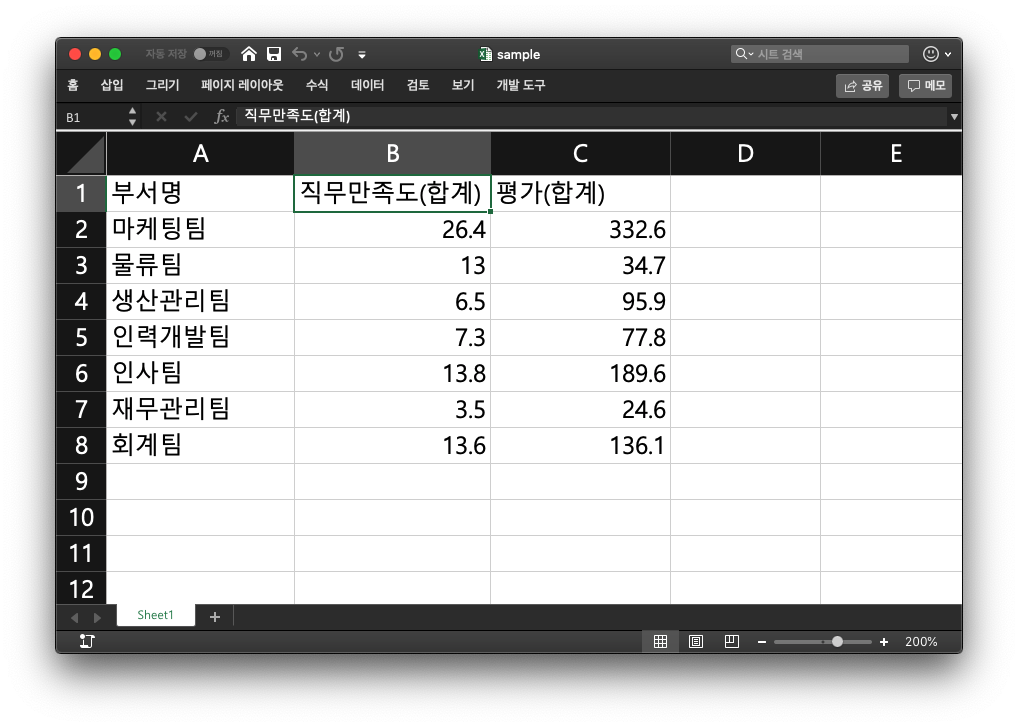
\includegraphics[scale=.33]{screenshot-excel}
\end{center}
\end{questiona}

\section{csv 파일}

스프레드시트 프로그램(Excel, LibreOffice Calc, etc.)은 고유의 포맷과 더불어 
csv (comma-separated version)라는 텍스트 형식의 파일 포맷을 읽고 쓸 수 있다.
csv는 plain text 파일이므로 이를 이용하여 Excel 데이터를 처리할 수 있다.

엑셀에서 “다른 이름으로 저장”을 선택하면 저장할 수 있는 형식 중에 CSV가 있다. 
기본 열 분리자는 쉼표(,)이다.
또는 “탭으로 분리된 텍스트”를 선택하여 \verb|*.txt|로 저장할 수 있는데 이것도 일종의
csv 포맷으로 본다. 
LibreOffice Calc는 csv 저장시에 분리자를 선택하는 옵션이 있을 것이다.

우리는 \verb|xlsx2csv|라는 유틸리티를 사용하려 한다. 이것은 다음과 같이 하여
설치할 수 있다. \verb|pip|은 버전에 맞는 명령을 주면 되고 python과 pip이
설치되어 있어야 한다.
\begin{verbatim}
pip install xlsx2csv
\end{verbatim}
우분투 18.04에서 
\begin{verbatim}
sudo apt install xlsx2csv
\end{verbatim}
로 되었던 기억이 있다.

열 분리자를 무엇으로 하면 좋을까? csv라는 이름은 “쉼표”임을 강력히 내세우고 있지만
\LaTeX{} 상황에서 쉼표는 생각을 좀 많이 해야 한다. 왜냐하면 텍스트 중에 쉼표가 
들어 있다면 그것을 열 분리자와 구분하기 위해 모두 \verb|{,}|로 묶어주는 번거로운
일을 감수해야 하기 때문이다.

그러나 텍스트 속의 쉼표 문제가 전혀 발생하지 않는다면 쉼표로 구분하는 것이 좋은데
각 행을 clist로 간단히 처리할 수 있을 것이기 때문이다.

열 분리자를 \verb|tab| 문자(\verb|\t|)로 하는 방법도 있다. 이호재 선생같은 경우
이 형식을 “tab separated version”이라고 TSV라고 부르기도 하는데 본질은 여전히 csv이므로
그렇게까지 구별해서 부를 이유가 있는지 모르겠고 아무튼 

\begin{verbatim}
xlsx2csv sample.xlsx sample.csv
xlsx2csv -d tab sample.xlsx sample.csv
\end{verbatim}

윗줄은 쉼표로 분리된 파일을, 아랫쪽은 tab으로 분리된 파일을 얻는다. 확장명은 둘 다
\verb|csv|이다.

쉼표로 분리하여 \verb|sample.csv|를 읽어들이면

\begin{examplebelow}
\verbatiminput{sample.csv}
\end{examplebelow}

\subsection{표 그리기}

한 줄씩 읽어서 표를 그리는 것은 간단할 것 같다. 한 번 해보자.

\begin{examplebelow}
\protected\def\newlinehline { \tabularnewline \hline }
\ExplSyntaxOn
\ior_new:N \l_xls_ior
\ior_open:Nn \l_xls_ior { sample.csv }
\tl_clear:N \l_tmpb_tl

\ior_str_map_inline:Nn \l_xls_ior
{
    \tl_set:Nn \l_tmpa_tl { #1 }
    \tl_replace_all:Nnn \l_tmpa_tl {, } { & }
    \regex_replace_all:nnN { $ } { \c{newlinehline } } \l_tmpa_tl 
    
    \tl_put_right:Nx \l_tmpb_tl { \l_tmpa_tl }
}

\ior_close:N \l_xls_ior

\begin{tabular}{|c|c|c|}
\hline
\l_tmpb_tl
\end{tabular}
\ExplSyntaxOff
\end{examplebelow}

위의 지나치게 간단한 해법은 다음 조건이 충족되었기 때문에 문제를 일으키지 않는다.
(1) 각 셀의 텍스트에 쉼표(,)가 없다.
(2) 각 셀의 텍스트에 앰퍼선드(\&)가 없다.
(3) 각 셀의 텍스트에 \LaTeX{} 명령이 없다.

\verb|\ior_str_...|으로 읽어온 이유는 이런 류의 외부 파일에는 \LaTeX 이 불평하기 쉬운
문자들 (\verb|#|, \verb|^|, \verb|_|, \verb|%| 등)이 포함되어 있을 가능성이 매우 높기 
때문이다. 이런 문자들을 에러없이 처리하려면 string으로 읽어오는 것이 좋다. 단 string으로
읽어오면 \TeX{} 명령이 포함되어 있을 때 이것이 실행되지 않는다.

\subsection{csv의 셀 분리}

B2 셀의 값을 얻으려 한다. 여기서 생각해보아야 할 것은 

\ATonum 1 데어터 전체의 각 행을 하나씩 clist에 넣어두고 그 $m$번째 clist의 $n$번째 item을 출력하는 방법

\ATonum 2 파일을 $m$행까지 읽어가서 그 행의 $n$번째 item을 출력하는 방법

둘 가운데 어느 것이 효율적이겠느냐 하는 것이다. 우리의 지금 샘플과 같이 행이 몇 되지 않는
csv의 경우는 어떤 것이든 별 차이 없겠지만 행이 아주 많은 table이라면 그 모두를 clist에 넣는 것은
비효율적이다. 또 특정 셀의 값을 알아내는 명령이 얼마나 자주 호출되느냐도 중요한데 clist에 저장해두는
것은 이런 호출이 매우 자주 일어날 때라면 오히려 나을 수도 있을 것이다.

주어진 행까지 파일을 읽어가서 해당 행 하나만 얻는 방법으로 해보자.

\begin{examplebelow}
\ExplSyntaxOn

\int_new:N \l_col_int
\int_new:N \l_row_int

\NewDocumentCommand \ShVal { m m }
{
    \int_set:Nn \l_col_int { \int_from_alph:n { #1 } }
    \int_set:Nn \l_row_int { #2 }
    
    \ior_open:Nn \l_xls_ior { sample.csv }
    
    \int_zero:N \l_tmpa_int 
    
    \ior_str_map_inline:Nn \l_xls_ior
    {
        \int_incr:N \l_tmpa_int
        
        \int_compare:nT { \l_tmpa_int == \l_row_int }
        {
             \tl_set:Nn \l_mthline_tl { ##1 }
             \ior_map_break:
        }
    }
    
    \ior_close:N \l_xls_ior

    \seq_set_from_clist:NN \l_a_seq \l_mthline_tl
    
    \seq_item:Nn \l_a_seq { \l_col_int }
}
\ExplSyntaxOff

\ShVal{B}{4}

\end{examplebelow}

이번에는 각 행을 모두 각각의 seq에 넣어보겠다.

\begin{examplebelow}
\ExplSyntaxOn

\NewDocumentCommand \ShVal { m m }
{
    \ior_open:Nn \l_xls_ior { sample.csv }
    
    \int_zero:N \l_row_int
    
    \ior_str_map_inline:Nn \l_xls_ior
    {
        \int_incr:N \l_row_int
        \seq_set_from_clist:cn { l_ \int_to_roman:n { \l_row_int } _ seq }
        { ##1 }
    }
    
    \ior_close:N \l_xls_ior
    
    \seq_if_exist:NT \l_i_seq { \int_set:Nn \l_col_int { \seq_count:N \l_i_seq } }
    
    \seq_item:cn { l_ \int_to_roman:n { #2 } _ seq }
    { \int_from_alph:n { #1 } }
    \c_space_token (
    \(
        \int_use:N \l_row_int \times \int_use:N \l_col_int
    \)
    )
}

\ExplSyntaxOff

\ShVal{C}{2}

\end{examplebelow}

위의 코드 중 재미있는 것은 \verb|\ShVal|이 불리고 나면 \verb|\l_col_int|와 
\verb|\l_row_int|가 이 table의 열과 행의 수를 보관하고 있다는 것이다. 
출력의 괄호 안에 적어보았다. 이 int 변수를 사용해서 명령 인자가 행과 열의 범위를
벗어나는지 검사하여 에러 처리를 할 수 있다.

그리고 눈여겨 볼 것은 \verb|\tl_set:Nn|과 같이 \verb|\seq_set_...| 함수도
만약 해당 seq가 \verb|new| 되어 있지 않으면 새로 만들고 설정해준다.
위와 같은 코드에서 \verb|\seq_new:N|를 일일이 해야 한다면 그것도 귀찮은 일이었을 것이다.


\subsection{csv와 \LaTeX}

\LaTeX{} 패키지 가운데 csv를 다루는 것은 다음과 같은 것이 있다: \textsf{csvsimple}, 
\textsf{datatool}, \textsf{pgfplotstable}.
이 중 csv뿐만 아니라 제법 본격적인 데이터베이스 도구를 제공하려는 야심찬 패키지가 \textsf{datatool}이고
\textsf{pgfplotstable}은 csv를 table로 그려주는 데 특화되어 있으며 일반적인 의미에서
csv를 적절하게 다루는 데는 \textsf{csvsimple}이 좋다고 본다.

이미 테스트해본 대로 csv를 expl3로 다루는 것은 매우 쉽다. 굳이 패키지에 의존하지 않고도
간단한 작업은 얼마든지 해낼 수 있을 것이다.

\vfill

\begin{questionp}
\fbox{기본} \bangotsuite.
첨부하는 파일 \verb|homework.xlsx|는 회원 주소록이다. 이 데이터로부터
가로 7cm인 박스 안에 우편번호, 주소, 이름을 인쇄하여 잘라서 봉투에 붙일 수
있게 A4 용지에 여러 개를 인쇄하여라. 절취선은 별도로 그리지 않아도 좋다.

\medskip

\leavevmode\fbox{\begin{minipage}{7cm}
\hspace*{1cm}    ~\\
\hspace*{1cm}	25467 \\
\hspace*{1cm}	강원도 강릉시 강문동 *** 번지 \\[5pt]
\hspace*{1cm}	\hspace*{4em} \makebox[5em][s]{\textsf{\Large 가 각 간}} 귀하 \\
\end{minipage}}

\end{questionp}


\vfill
\hfill Nova de Hi.


\end{document}

